\documentclass{beamer}
\usepackage{mathtools}
\usepackage{amsmath}
\usetheme{CambridgeUS}

\title{Receive Antenna Selection in MIMO Systems}
\author{Sandeep H M \and Dinesh Kumar Sonkar}
\date{\today}
\subject{EE5327 - Optimization}

\begin{document}

\begin{frame}
  \titlepage
\end{frame}

\section{Introduction}
\begin{frame}{Introduction}
Multiple-Input and Multiple-Output(MIMO) is a method for multiplying the capacity of a radio link using multiple transmission and receiving antennas to exploit multipath propagation\\
\vskip 0.2in
MIMO has become an essential element of wireless communication standards like WiFi,3G,4G and 4G-LTE.\\
\vskip 0.2in
A limiting factor in it's deployment is the cost of multiple analog chains at the receiver end.\\
\vskip 0.2in
By Antenna selection,a limited number of transmit/receive chains are used, thereby bringing the cost
    
\end{frame}

\section{System Model}
\begin{frame}{System Model}
Received signal can be represented as 
\begin{equation*}
    x(k) =\sqrt{E_s}\boldsymbol{H}s(k)+ \boldsymbol{n}(k)
\end{equation*}
where\\
x(k) is a vector of size M$\times$1. It represents the $k^{th}$ sample of the signals collected at the M receive antennas.\\
\vskip 0.1in
s(k) is a vector of size N$\times$1. It represents the $k^{th}$ sample of the signals transmitted at the N transmit antennas.\\
\vskip 0.1in
$E_s$ is the average energy per receive antenna and per channel use\\
\vskip 0.1in
n(k)  is AWGN with energy $\frac{N_0}{2}$\\
\vskip 0.1in
\textbf{H} is the M$\times$N channel matrix.The entries of \textbf{H} are assumed to be zero-mean circularly symmetric complex Gaussian (ZMCSCG), such that the covariance matrix of any two columns of \textbf{H} is a scaled identity matrix.
\end{frame}
\section{Receive Antenna Selection In MIMO Systems}
\begin{frame}{Receive Antenna Selection In MIMO Systems}
`\textbf{Objective} - Select receive antenna to maximize capacity.\\
The capacity of a system is given by the formula
\begin{equation*}
    C(\boldsymbol{H})=\log_{2}\text{det}(\boldsymbol{I}_{N} + \gamma\boldsymbol{R}_{ss}\boldsymbol{H}^{H}\boldsymbol{H})
\end{equation*}
where\\
\vskip 0.2in
\gamma = \textstyle\frac{E_s}{N_0}
\newline
\newline
\mathbf{R}$_{ss}$ = E[s(k)s(k)$^H$] is the co-variance matrix of the transmitted signals with trace(\textbf{R}$_{ss}$)=1
\end{frame}

\begin{frame}{}
When only M'$<$M receive antennas are used, the capacity becomes a function of the antennas chosen.\\
\vskip 0.2in
We represent the indices of the selected antennas by r =
[r$_1$, . . . , r$_{M'}$]\\
\vskip 0.2in
The effective channel matrix becomes \textbf{H}$_r$ which is a M'$\times$N matrix.\\
\vskip 0.2in
The channel capacity with antenna selection is given by
\begin{equation*}
    C_r(\boldsymbol{H}_r) = \log_{2}\text{det}(\boldsymbol{I}_{N} + \gamma\boldsymbol{R}_{ss}\boldsymbol{H}_{r}^{H}\boldsymbol{H}_{r})
\end{equation*}
\end{frame}

\section{ANTENNA SELECTION AS AN OPTIMIZATION PROBLEM}
\begin{frame}{Antenna Selection as an Optimization Problem}`
We define \Delta$_i$
\[ \Delta_i = 
     \begin{cases}
       \text{1,} & \quad\text{if}\quad i$^{th}$ antenna is selected\\
       \text{0,} &\quad\text{otherwise.} \\ 
     \end{cases}
\]

Now, consider an M$\times$M diagonal matrix $\mathbf{\Delta}$ that has $\Delta_i$ as its diagonal entries.\\
Let us denote F =  $\mathbf{\Delta}$H.\\
F can be written as \textbf{H}$_r$ with (M-M') zero rows appended
to it and left multiplied by a M ×M row-permutation matrix P. Thus,
\begin{equation*}
    \boldsymbol{F} = \boldsymbol{P}
     \begin{bmatrix}
    \boldsymbol{H}_r\\
    0 _{(M-M')\times N}
\end{bmatrix}
= \boldsymbol{P}\widetilde{\boldsymbol{H}_{r}}
\end{equation*}
\end{frame}

\begin{frame}{}
Since P is a permutation matrix, \textbf{P$^H$}\textbf{P} = \textbf{I}$_M$.
\begin{align*}
\textbf{F}^H\textbf{F} &= \widetilde{\boldsymbol{H}_{r}}^H\textbf{P}^H\textbf{P}\widetilde{\boldsymbol{H}_{r}}\\
&= \widetilde{\boldsymbol{H}_{r}}^H\widetilde{\boldsymbol{H}_{r}}\\
&= \textbf{H}_r^H\textbf{H}_r
\end{align*} 
The channel capacity as a function of $\mathbf{\Delta}$ is
\begin{align*}
\mathnormal{C}_r(\mathbf{\Delta}) &=\log_{2}\text{det}(\mathbf{I}_N + \gamma\textbf{F}^H\textbf{F})\\
&= \log_{2}\text{det}(\mathbf{I}_N + \gamma\textbf{H}^H\mathbf{\Delta}^H\mathbf{\Delta}\textbf{H})
\end{align*}
\end{frame}

\begin{frame}{}
Since $\mathbf{\Delta}$ is a diagonal matrix with entries either 0 or 1\\
$$\mathbf{\Delta}^H\mathbf{\Delta}=\mathbf{\Delta}$$
The MIMO channel capacity with antenna selection can be re-written as
\begin{align*}
\mathnormal{C}_r(\mathbf{\Delta}) &=\log_{2}\text{det}(\mathbf{I}_N + \gamma\textbf{H}^H\mathbf{\Delta}\textbf{H})
\end{align*}
Using the identity det(\textbf{I$_m$} + \textbf{A}\textbf{B}) = det(\textbf{I}$_n$ + \textbf{B}\textbf{A}) we get
\begin{align*}
\mathnormal{C}_r(\mathbf{\Delta}) &=\log_{2}\text{det}(\mathbf{I}_M + \gamma\mathbf{\Delta}\textbf{H}\textbf{H}^H)
\end{align*}
\end{frame}

\begin{frame}{}
Maximize 
\begin{align*}
\mathnormal{C}_r(\mathbf{\Delta}) &=\log_{2}\text{det}(\mathbf{I}_M + \gamma\mathbf{\Delta}\textbf{H}\textbf{H}^H)
\end{align*}
subject to
$$0\leq\Delta_{i}\leq1,\enspace i=1,2,...,M$$
$$trace(\mathbf{\Delta})=\sum_{i=1}^{M} \Delta_i = M'$$
\end{frame}
 
 \section{Optimization in JMMSE receiver}
\begin{frame}{Optimization in JMMSE receiver}
The capacity acheivable is $\mathnormal{C}_{\mathnormal{J}}(\mathbf{H})$ is
$$\mathnormal{C}_{\mathnormal{J}}(\mathbf{H}) = \sum_{k=1}^{N} \log_{2}(1 + \rho_{k}^2)$$
where 
$$\rho_{k}^2 = \Big[\big(\mathbf{I}_N + \gamma\textbf{H}^H\textbf{H}\big)^{-1}\Big]_{k,k}^{-1}$$
is the SINR of the kth output stream of the MMSE receiver.\\
\end{frame}

\begin{frame}{}
Since $$\mathbf{H}_r^H\mathbf{H}_r = \mathbf{H}^H\mathbf{\Delta}\mathbf{H}$$
The capacity of the JMMSE architecture with receive antenna selection is given by
$$\mathnormal{C}_{\mathnormal{J_r}}(\mathbf{H}) = \sum_{k=1}^{N} \log_{2}(1 + \Tilde{\rho_{k}}^2)$$
where
$$\Tilde{\rho_{k}}^2 = \Big[\big(\mathbf{I}_N + \gamma\textbf{H}^H\mathbf{\Delta}\textbf{H}\big)^{-1}\Big]_{k,k}^{-1}$$
\end{frame}

\begin{frame}{}
Maximize 
$$\mathnormal{C}_{\mathnormal{J_r}}(\mathbf{H}) = \sum_{k=1}^{N} \log_{2}(1 + \Tilde{\rho_{k}}^2)$$
where
$$\Tilde{\rho_{k}}^2 = \Big[\big(\mathbf{I}_N + \gamma\textbf{H}^H\mathbf{\Delta}\textbf{H}\big)^{-1}\Big]_{k,k}^{-1}$$
subject to
$$0\leq\Delta_{i}\leq1,\enspace i=1,2,...,M$$
$$trace(\mathbf{\Delta})=\sum_{i=1}^{M} \Delta_i = M'$$
\end{frame}

\section{Result}

\begin{frame}{Result}
Receive antenna subset selection has been approximated by a constrained convex relaxation  that can be solved using standard low
complexity techniques\\
\vskip 0.1in
The selection algorithm gives an Ergodic capacity which is very close to the optimal one
\begin{figure}[h]
\centering
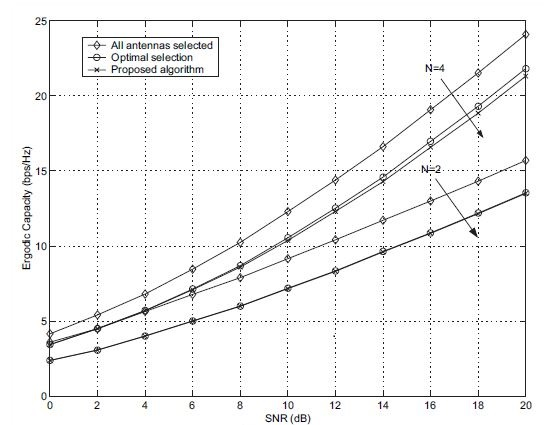
\includegraphics[width=0.3\textwidth]{JMMSE_SNR.JPG}
\caption{Ergodic capacity v/s SNR (N$_\gamma$) for JMMSE, M = 6, N = 2,4 M' = N}
\end{figure}
\end{frame}


\end{document}
